\documentclass[12pt,a4paper]{article}

% ── packages ───────────────────────────────────────────────────────────────
\usepackage[utf8]{inputenc}
\usepackage[T1]{fontenc}
\usepackage[english]{babel}
\usepackage{graphicx}
\usepackage{booktabs}
\usepackage{amsmath}
\usepackage{hyperref}
\usepackage{geometry}
\usepackage{caption}
\usepackage{float}

\geometry{margin=2.5cm}

\title{Custom-WikiCS Graph Analysis -- Part 2\\[4pt]
\large Connected Components, Centrality Measures \& Community Detection}
\author{}
\date{\today}

\begin{document}
\maketitle

% ═══════════════════════════════════════════════════════════════════════════
\section{Introduction}
% ═══════════════════════════════════════════════════════════════════════════

This report presents the second phase of structural analysis on the
Custom-WikiCS graph, a directed graph derived from Wikipedia computer-science
articles.  Each node represents an article and each directed edge represents a
hyperlink from one article to another.

The analyses covered are:
\begin{enumerate}
    \item Connected component decomposition (weakly and strongly connected).
    \item Centrality measures: Degree, Betweenness, Closeness and PageRank.
    \item Community detection using Louvain and Infomap algorithms, with a
          comparative discussion.
\end{enumerate}

\begin{itemize}
    \item \textbf{Nodes:} 11\,701
    \item \textbf{Directed edges:} 291\,039
    \item \textbf{Undirected edges:} 216\,123
\end{itemize}

% ═══════════════════════════════════════════════════════════════════════════
\section{Connected Components}
% ═══════════════════════════════════════════════════════════════════════════

A \emph{weakly connected component} (WCC) ignores edge direction: two nodes
belong to the same WCC if there exists any undirected path between them.  A
\emph{strongly connected component} (SCC) requires a directed path in
\emph{both} directions.

\begin{table}[H]
\centering
\caption{Connected component statistics.}
\label{tab:components}
\begin{tabular}{lrrl}
\toprule
\textbf{Metric} & \textbf{Count} & \textbf{Largest} & \textbf{Coverage} \\
\midrule
Weakly Connected Components  & 356   & 11\,311 nodes & 96.7\% \\
Strongly Connected Components & 2\,510 & 9\,062 nodes  & 77.4\% \\
\bottomrule
\end{tabular}
\end{table}

The graph contains \textbf{356~weakly connected components}, with the largest
WCC covering 11\,311 of the 11\,701~nodes ($96.7\%$).  This indicates that the
vast majority of articles are reachable from one another when edge direction is
ignored; only a small fringe of 390~nodes sits in isolated or tiny components.

The number of \textbf{strongly connected components} rises to 2\,510.  The
largest SCC encompasses 9\,062~nodes ($77.4\%$), meaning that more than
three-quarters of all articles can reach each other via directed hyperlink
paths.  The gap between the WCC and SCC sizes ($96.7\%$ vs.\ $77.4\%$)
reveals a substantial ``periphery'' of roughly 2\,249~nodes that are linked
\emph{to} the core but do not themselves link back, forming a directed
in-component or out-component around the giant SCC.

% ═══════════════════════════════════════════════════════════════════════════
\section{Centrality Measures}
% ═══════════════════════════════════════════════════════════════════════════

Four centrality metrics were computed to capture different aspects of node
importance.  Degree and PageRank were evaluated on the \emph{directed} graph;
Betweenness and Closeness were computed on the \emph{undirected} version for
computational efficiency and interpretability.

\subsection{Summary Statistics}

\begin{table}[H]
\centering
\caption{Centrality statistics across all 11\,701 nodes.}
\label{tab:centrality}
\begin{tabular}{lrrrrr}
\toprule
\textbf{Metric} & \textbf{Min} & \textbf{Max} & \textbf{Mean} & \textbf{Median} & \textbf{Std} \\
\midrule
Degree Centrality      & 0.000000 & 0.296923 & 0.004252 & 0.001197 & 0.007580 \\
Betweenness Centrality & 0.000000 & 0.203581 & 0.000161 & 0.000008 & 0.002308 \\
Closeness Centrality   & 0.000000 & 0.534778 & 0.314644 & 0.323041 & 0.069561 \\
PageRank               & 0.000013 & 0.009963 & 0.000085 & 0.000032 & 0.000205 \\
\bottomrule
\end{tabular}
\end{table}

\paragraph{Degree Centrality.}
The mean degree centrality is only $0.0043$, confirming a sparse graph where
nodes are connected to a tiny fraction of all others.  The maximum of $0.2969$
indicates that the most connected node links to roughly $30\%$ of the network,
while the median ($0.0012$) is roughly $3$--$4\times$ lower than the mean---a
signature of a heavy-tailed degree distribution.

\paragraph{Betweenness Centrality.}
Betweenness is even more concentrated: the mean is $0.000161$ with a maximum
of $0.2036$.  The vast majority of shortest paths therefore pass through a
handful of bridge nodes.  The median is extremely close to zero ($0.000008$),
showing that most nodes play virtually no brokerage role.

\paragraph{Closeness Centrality.}
Closeness values are more evenly spread (std~$=0.0696$).  The mean of $0.3146$
and median of $0.3230$ indicate that a typical node can reach all others in
roughly $1/0.31 \approx 3.2$ hops on average.  The maximum closeness ($0.5348$)
shows that the most central node is, on average, fewer than two hops away from
every other node.  Nodes with closeness~$= 0$ reside in components disconnected
from the giant component.

\paragraph{PageRank.}
PageRank assigns a probability of $0.0001$ to the average node, with a maximum
of $0.0100$.  The ratio $\text{max}/\text{mean} \approx 117$ reflects the
extreme concentration of link authority in a few hub articles.  The standard
deviation ($0.000205$) exceeds twice the mean, confirming a strongly skewed
distribution.

\subsection{Centrality Distributions}

Figure~\ref{fig:centrality} shows the distribution histograms for all four
centrality metrics.

\begin{figure}[H]
    \centering
    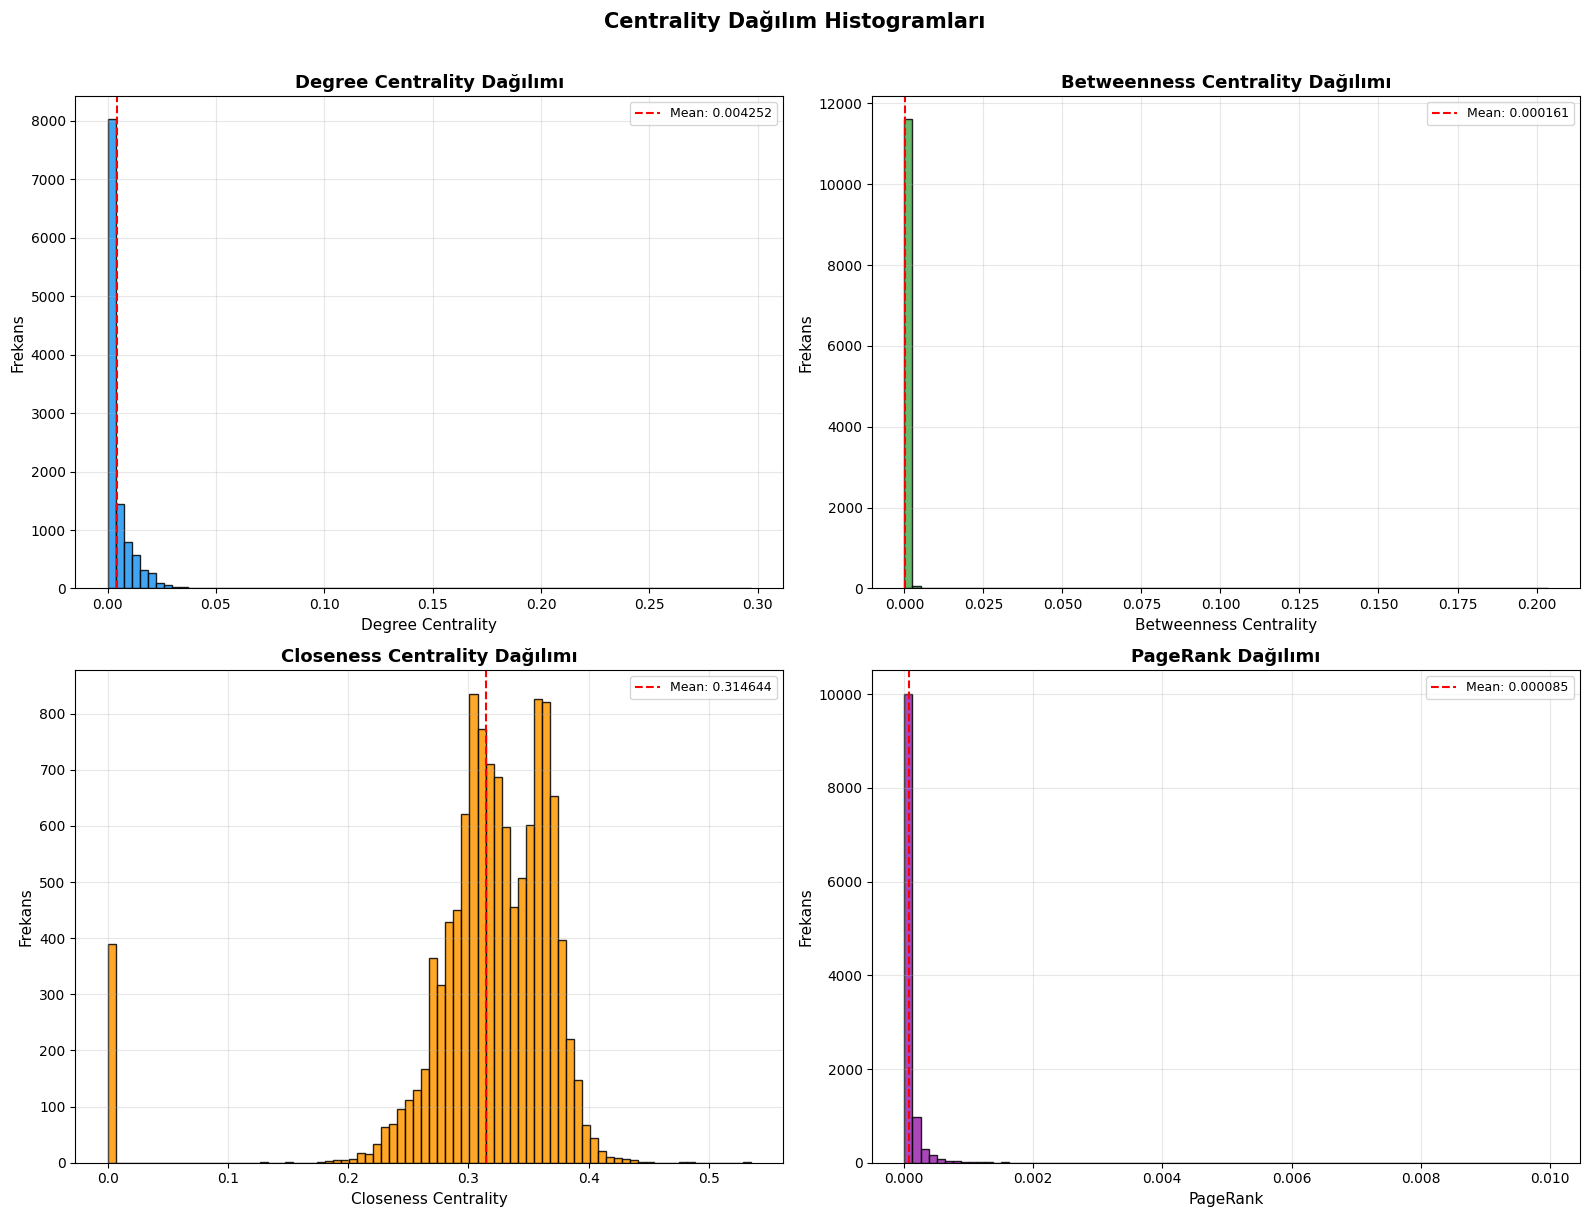
\includegraphics[width=\textwidth]{img-2/centrality.png}
    \caption{Centrality distribution histograms: Degree (top-left),
             Betweenness (top-right), Closeness (bottom-left) and
             PageRank (bottom-right).  Red dashed lines indicate the mean.}
    \label{fig:centrality}
\end{figure}

All four distributions are right-skewed.  Degree, Betweenness and PageRank
concentrate the bulk of their mass near zero with long tails toward the
right, which is characteristic of scale-free networks.  Closeness Centrality
is the exception: its histogram is approximately bell-shaped and centred
around $0.32$, indicating that most nodes in the giant component have
comparable average path lengths, while the left tail captures nodes in
smaller or peripheral components.

% ═══════════════════════════════════════════════════════════════════════════
\section{Community Detection}
% ═══════════════════════════════════════════════════════════════════════════

Two widely-used community detection algorithms---\textbf{Louvain} and
\textbf{Infomap}---were applied to the undirected version of the graph.
Both aim to partition nodes into densely connected groups (communities),
but they optimise different objective functions: Louvain maximises modularity,
while Infomap minimises the map equation (description length of a random walk).

\subsection{Louvain Algorithm}

\begin{table}[H]
\centering
\caption{Louvain community detection results.}
\label{tab:louvain}
\begin{tabular}{lr}
\toprule
\textbf{Statistic} & \textbf{Value} \\
\midrule
Modularity          & 0.650354 \\
Number of communities & 373 \\
Min community size  & 1 \\
Max community size  & 1\,971 \\
Mean community size & 31.37 \\
Median community size & 1.0 \\
Std deviation       & 176.52 \\
\bottomrule
\end{tabular}
\end{table}

Louvain achieves a modularity of \textbf{0.6504}, which indicates a strong
community structure (values above $0.3$ are generally considered significant).
The algorithm identifies 373~communities, but the size distribution is
extremely skewed: the median community size is just~1 (i.e., many singleton
communities), while the largest community contains 1\,971~nodes---nearly
$17\%$ of the entire graph.  The high standard deviation ($176.52$) reflects
this imbalance: a few large communities coexist with hundreds of tiny or
singleton groups.

\begin{figure}[H]
    \centering
    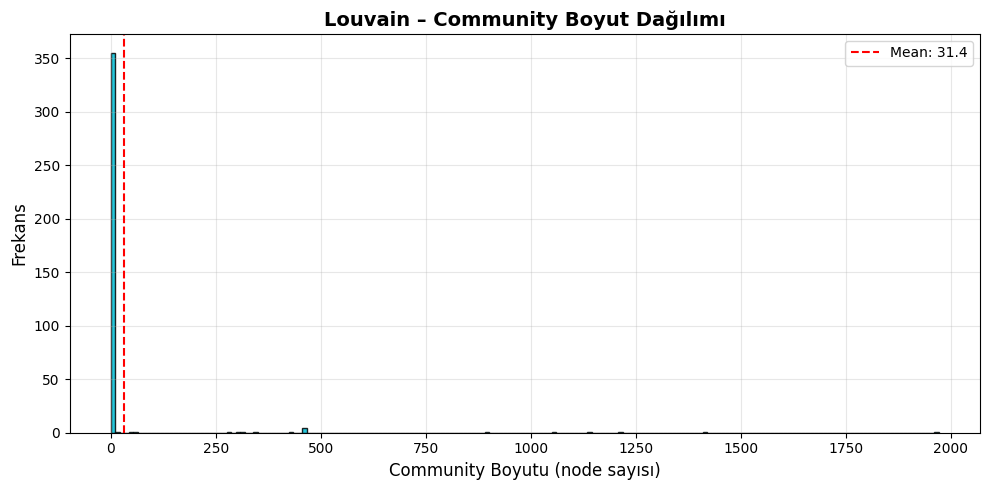
\includegraphics[width=0.85\textwidth]{img-2/louvain-community.png}
    \caption{Louvain community size distribution.  The red dashed line marks
             the mean size ($31.4$).}
    \label{fig:louvain}
\end{figure}

Figure~\ref{fig:louvain} confirms the heavy-tailed nature of the community
size distribution.  The overwhelming majority of communities (over~350) are
clustered near the origin with fewer than~50 nodes, while a handful of
large communities extend the histogram tail past 1\,500 nodes.  This pattern
suggests that the graph has a small number of broad topical clusters (e.g.,
``Machine Learning'', ``Algorithms'', ``Programming Languages'') that attract
many articles, alongside numerous narrowly-scoped micro-topics that form
only one or two articles each.

\subsection{Infomap Algorithm}

\begin{table}[H]
\centering
\caption{Infomap community detection results.}
\label{tab:infomap}
\begin{tabular}{lr}
\toprule
\textbf{Statistic} & \textbf{Value} \\
\midrule
Modularity          & 0.599823 \\
Number of communities & 596 \\
Min community size  & 1 \\
Max community size  & 837 \\
Mean community size & 19.63 \\
Median community size & 1.0 \\
Std deviation       & 73.56 \\
\bottomrule
\end{tabular}
\end{table}

Infomap yields a modularity of \textbf{0.5998}, slightly lower than Louvain's
value.  It discovers 596~communities---roughly $60\%$ more than Louvain.  The
maximum community size drops from 1\,971 to 837, and the mean from 31.37 to
19.63, indicating that Infomap tends to split the graph into finer-grained
modules.  The median remains at~1, confirming the persistence of many singleton
communities, and the standard deviation decreases to $73.56$.

\begin{figure}[H]
    \centering
    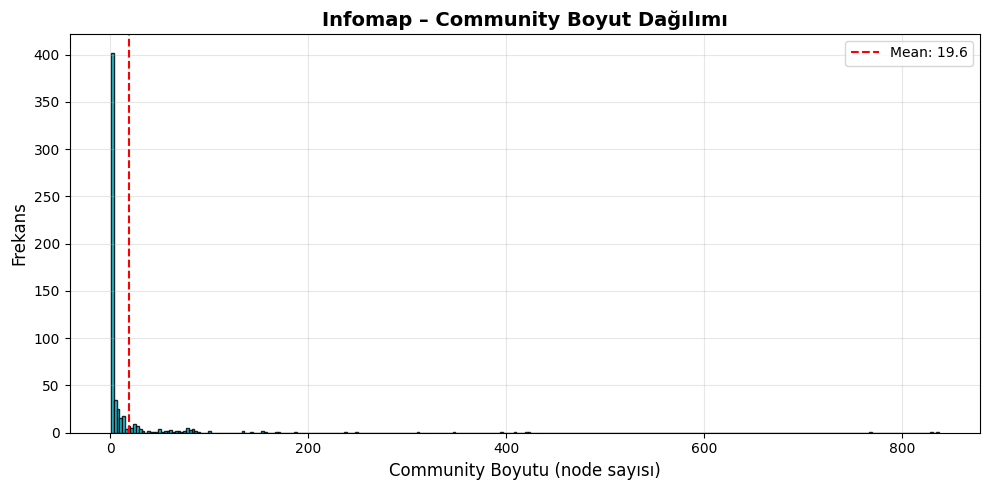
\includegraphics[width=0.85\textwidth]{img-2/infomap.png}
    \caption{Infomap community size distribution.  The red dashed line marks
             the mean size ($19.6$).}
    \label{fig:infomap}
\end{figure}

Figure~\ref{fig:infomap} shows that Infomap's distribution, while still
heavily right-skewed, has a shorter tail (max~837 vs.\ 1\,971) and more
communities in the 10--100 range than Louvain.  The Infomap algorithm's
information-theoretic approach captures tighter flow-based modules: it
identifies cohesive subgraphs where a random walker tends to stay for
extended periods, rather than simply maximising the ratio of internal to
external edges.

\subsection{Louvain vs.\ Infomap Comparison}

\begin{table}[H]
\centering
\caption{Louvain vs.\ Infomap comparison.}
\label{tab:comparison}
\begin{tabular}{lrrrrrrr}
\toprule
\textbf{Algorithm} & \textbf{Modularity} & \textbf{Communities} & \textbf{Min} & \textbf{Max} & \textbf{Mean} & \textbf{Median} & \textbf{Std} \\
\midrule
Louvain & 0.6504 & 373 & 1 & 1\,971 & 31.37 & 1.0 & 176.52 \\
Infomap & 0.5998 & 596 & 1 & 837   & 19.63 & 1.0 & 73.56  \\
\bottomrule
\end{tabular}
\end{table}

The key differences are:

\begin{itemize}
    \item \textbf{Modularity:} Louvain achieves a higher modularity ($0.6504$
          vs.\ $0.5998$), which is expected since it directly optimises this
          metric.  However, higher modularity does not necessarily imply
          ``better'' communities; Infomap optimises a different (information-
          theoretic) objective that can capture more nuanced flow patterns.

    \item \textbf{Granularity:} Infomap produces roughly $60\%$ more
          communities ($596$ vs.\ $373$).  Its largest community ($837$~nodes)
          is less than half the size of Louvain's largest ($1\,971$~nodes).
          Infomap therefore provides a more fine-grained partition, which may
          be preferable for downstream tasks that benefit from homogeneous,
          tightly-knit groups.

    \item \textbf{Size distribution:} Both algorithms yield many singleton
          communities (median~$= 1$), but Louvain's standard deviation is
          more than twice that of Infomap ($176.52$ vs.\ $73.56$), indicating
          a more uneven split.  Louvain creates a few very large
          ``super-communities'' alongside many micro-communities, whereas
          Infomap distributes nodes more evenly among medium-sized clusters.

    \item \textbf{Interpretation:} Louvain's modularity-based approach groups
          nodes by maximising internal edge density relative to a null model.
          Infomap's random-walk--based approach detects regions where
          information flow is self-contained.  For a knowledge graph like
          Custom-WikiCS, Infomap's finer decomposition may better capture
          thematic sub-topics (e.g., separating ``Deep Learning'' from the
          broader ``Machine Learning'' cluster), while Louvain's coarser
          grouping may better reflect high-level disciplinary boundaries.
\end{itemize}

% ═══════════════════════════════════════════════════════════════════════════
\section{Conclusion}
% ═══════════════════════════════════════════════════════════════════════════

The Custom-WikiCS graph exhibits a well-connected core: $96.7\%$ of nodes
belong to a single weakly connected component and $77.4\%$ to a single
strongly connected component.  Centrality analysis reveals a scale-free--like
structure where a small elite of hub articles dominates degree, betweenness
and PageRank rankings, while closeness is more uniformly distributed across
the giant component.

Community detection confirms the presence of meaningful modular structure
(modularity~$> 0.6$).  Louvain produces fewer, larger communities with higher
modularity, while Infomap yields more numerous, smaller and more uniform
communities.  Both algorithms agree on a heavy-tailed community size
distribution with many singleton or very small communities alongside a few
dominant clusters.  The choice between the two depends on the desired level
of granularity for downstream applications such as node classification or
graph neural network training.

\end{document}
